\documentclass[12pt,a4paper,oneside]{article} %% Dokumenten Parameter und Art des Dokuments
\usepackage[utf8]{inputenc} %% Diese Datei ist im utf8 Format dies ist hier damit Latex uns versteht
\usepackage[ngerman]{babel} %% Rechtschreib prüfung
\usepackage{hyperref}
\usepackage{amsmath} %% Packet zur verwendung Mathematischer Formeln
\usepackage{amsfonts}
\usepackage{amssymb} %% Packet zur verwendung Mathematischer Symbole
\usepackage{mathtools}
\usepackage{microtype} %% Sorgt für besseren umgang mit zu lange/kurzen Zeilen
\usepackage{pdfpages} %% Zum einfügen eines PDf dokuments
\title{TGI Serie 5}
\author{Bennet Bleßmann, Sven Korfmann}

\begin{document}
\maketitle

\section*{H1}

\subsection*{a)}

$(q_{0},0011,Z_{0}) \to (q_{1},011,OZ_{0}) \to (q_{1},11,0OZ_{0}) \to (q_{2},1,OZ_{0}) \to (q_{3},\varepsilon,Z_{0})$

\subsection*{b)}

Da $K_{\alpha}$ nur begrenzten Speicher hat akzeptiert $K_{\alpha}$ 

nur die Sprache $\{0^{n}1^{n}|n \in \mathbb{N}_{<\alpha}\}$.

\subsection*{c)}

\subsubsection*{Reguläre Sprachen lassen sich durch DKAS erkennen.}
Ein DKAS ist ein um $\varepsilon$-Transitionen und einen Kellerspeicher erweiterter DEA
somit ist jede reguläre Sprache durch einen DKAS erkennen.

\subsubsection*{Alle durch einen DKAS definierten Sprachen sind regulär.} 

Sei $K = (Q,\Sigma,\Gamma,\delta,Z_{0},q_{0},F,c)$ DKAS.

Da wir annehmen dürfen das für jedes $K$ mit $\varepsilon$-Transitionen

einen äquivalenter DKAS ohne $\varepsilon$-Transitionen existiert,

nehmen wir ab hier an das $K$ keine $\varepsilon$-Transitionen besitzt.

Im folgendem definieren wir einen zu $K$ äquivalenten DEA $m$,

was so mit zeigt das DKAS reguläre Sprachen definieren.

\paragraph{} Wir definieren

	$Q^{\prime} = Q \times \{x \in \Gamma^{*} | 1 \leq |x| < \alpha\}$
	
	$F^{\prime} = \{(q,k) \in Q^{\prime} | q \in F$, $k \in \Gamma^{*}\}$	
	
	$R \notin Q^ {\prime}$
	
	$q_{0}^{\prime} = (q_{0},Z_{0})$
	
	Für $(q,zr) \in Q'$ mit $|z| = 1$ und $a \in \Sigma$
	
	$\delta^{\prime}((q,zr),a) = 
\begin{cases*}
(q^{\prime},z^{\prime}r)  &, falls $\exists~(q^{\prime},z^{\prime}) \in \delta(q,a,z)$ \\
(q^{\prime},z^{\prime}zr) &, falls $\exists~(q^{\prime},z^{\prime}) \in \delta(q,a,\varepsilon)$ \\
R                         &, sonst 
\end{cases*} $

sowie

$\delta^{\prime}(R,a) = R$

$m = (Q^{\prime} \cup \{R\},\Sigma,\delta^{\prime},q_{0}^{\prime},F^{\prime})$




\section*{Aufgabe 2}

Sei $ p\in N_>0 $ Wähle $ w= 10^p(10)^p1^p0\#10^p(10)^p1^p0 $ Damit gilt $|w|>p$ sei $uxyzv=w$ sodass $|xz|>0 \wedge |xyz|<p$ dann gilt: \\
Wenn $\# \in x$ oder $ \# \in x$ dann gilt 
$ux^iyz^iv \not\in L$ für $i \in N_>1$ \\
Wenn $\# \in u$ oder $ \# \in v$ dann gilt 
$ux^iyz^iv \not\in L$ für $i \in N_>1$\\
Wenn $\# \in y$  dann gilt 
$ux^iyz^iv \not\in L$ für $i \in N_>1$\\

\section*{H3}

\subsection*{a)}
	
Sei $\Sigma$ Alphabet mit \textvisiblespace$ \notin \Sigma$ ,so dass $L = \Sigma^{*}$ unendliche Sprache.

Dann akzeptiert die Turing Maschine 
$T = (\{q_{0},q_{1}\},\Sigma,\Sigma \cup \{$\textvisiblespace$\},\delta,q_{0},\{q_{1}\})$ 

mit $\delta(q_{0},r) = \{(q_{1},r,L)\}$ für alle $r \in \Sigma \cup \{$\textvisiblespace$\}$ die Sprache L.

Also existiert eine Turing Maschine T

welche eine unendliche Sprache akzeptiert ohne 

das der Kopf sich um mehr als einen Schritt von der Startposition entfernt.

\subsection*{b)}

Im folgendem wird die Aussage 
\begin{quote}
	Zu jeder Turing Maschine $M_{1}$ existiert eine Turing Maschine $M_{2}$
	mit nur einem Zustand und $L(M_{1}) = L(M_{2})$.
\end{quote} widerlegt.

Sei $M_{1}$ eine Turing Maschine,

welche das Wort $a$ akzeptiert und das Wort $b$ verwirft.

Dann kann keine Turing Maschine $M_{2}$ existieren,

welche nur einen Zustand hat und für die $L(M_{1})=L(M_{2})$ gilt.

Da $M_{2}$ nur einem Zustand hätte könnte $M_{2}$ entweder alle Wörter akzeptiert

oder alle Wörter verwerfen.

Da für $M_{1}$ sowohl ein Wort akzeptiert als auch verworfen werden muss,

widerlegt dies die Aussage.

\subsection*{c)}

Die hier zu Beweisende Aussage wird durch die Turing Maschine T in a),
welche die Bedingung, dass sich der Kopf nur nach links Bewegt, erfüllt, widerlegt,
da $\varepsilon \in L(T)$, aber $\varepsilon \notin \Sigma^{+}$, und so mit nicht $L(T) \subseteq \Sigma^{+}$


\section*{Aufgabe 4}

\subsection*{a)}
Preudocode:
1. Wähle erstes Element ist es leer akzeptiere, wenn nicht Merke es dir und lösche das Original\\
2. Gehe ans ende des Wortes \\
3. Überprüfe ob es mit dem ersten Element übereinstimmt,
 wenn nicht verwerfe, ansonsten gehe zum Anfang des Wortes und zu 1\\ \\
$TN = \lbrace \lbrace q_0 ,q_1 ,q_2 ,q_3 ,q_4 , q_5 , q_acc , q_rej \rbrace , \lbrace 0,1 \rbrace , \lbrace \_ \rbrace , \delta , q_0 , \_ , \lbrace q_acc \rbrace \rbrace  $ \\

Mit$ \delta = \lbrace \\
 (q_0 , 1 \rightarrow q_1 , \_ , R), (q_0 , 0 \rightarrow q_4 , _, R), (q_0 , \_  \rightarrow q_1 , _, R),\\ (q_1 , 1 \rightarrow q_1 , 1, R), (q_1 , 0 \rightarrow q_1 , 0, R),(q_1 , \_ \rightarrow q_2 , _, L),\\ (q_2 , 1 \rightarrow q_3 , \_ ,L),(q_2 , \_ \rightarrow q_rej , \_ ,L),(q_2 , 0 \rightarrow q_rej , \_ ,L),\\(q_3 , 0 \rightarrow q_3 , 0 ,L),(q_3 ,1 \rightarrow q_3 , 1 ,L),(q_3 , \_ \rightarrow q_0 , \_ ,R),\\ (q_4 , 1 \rightarrow q_4 , 1, R), (q_4 , 0 \rightarrow q_4 , 0, R),(q_4 , \_ \rightarrow q_5 , _,L),\\(q_5 , 0 \rightarrow q_3 , \_ ,L),(q_5 , \_ \rightarrow q_rej , \_ ,L),(q_5 , 1 \rightarrow q_rej , \_ ,L) \rbrace $
\subsection*{b)}
1. Zähle Elemente des Ersten Bandes im zweiten Band. \\
2. Ist die Zahl ungerade lehne Eingabe ab wenn nicht halbiere sie. \\
3. Speichere erste Hälfte des Wortes im Zweiten Band.\\
4. Prüfe ob Zweite Hälfte des Wortes Mit dem Oberen Band Übereinstimmmt, wenn ja akzeptiere wenn nei lehne ab. \\

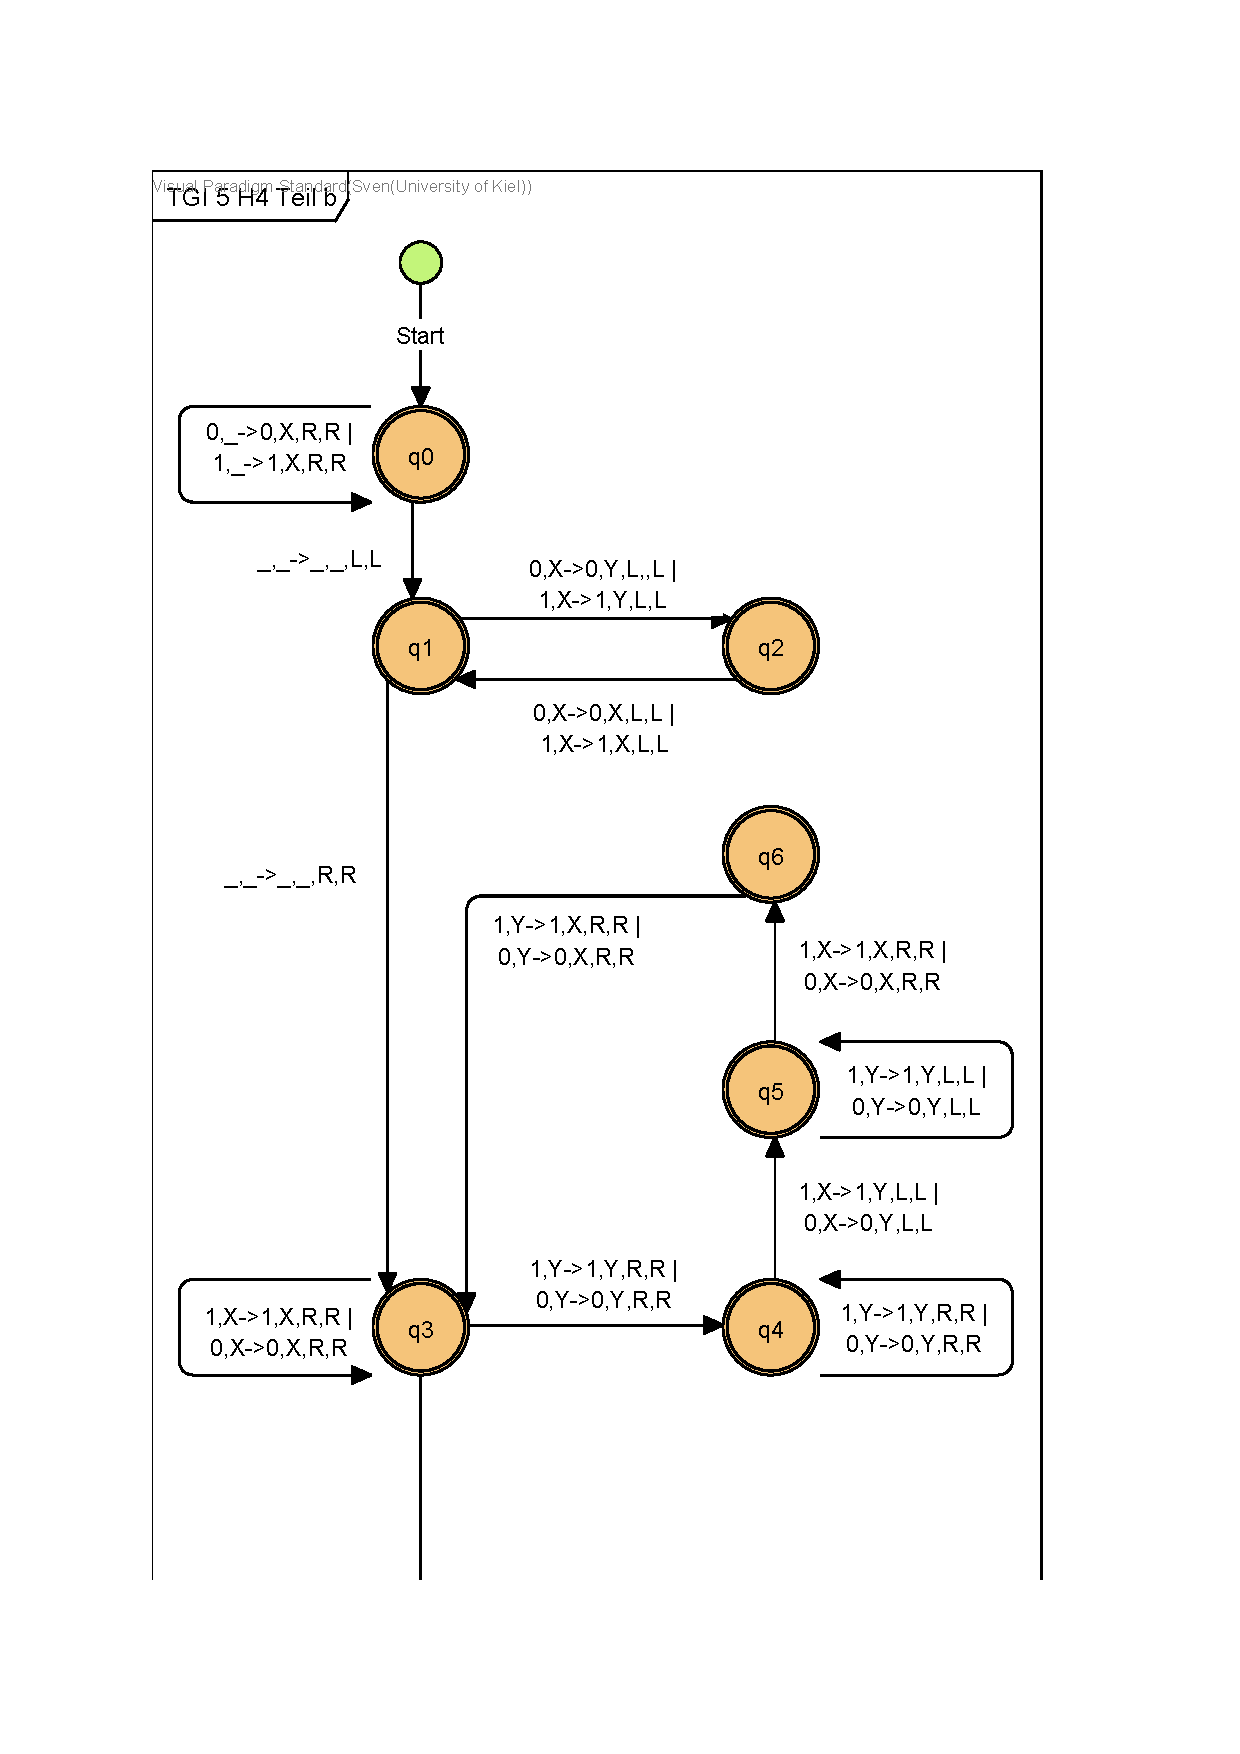
\includepdf[pages=-]{TGI_5_teil_b.pdf}
 

\subsection*{c)}
1. Kopiere Wort bis \# in das 2. Band. \\
2. Addiere 1 zu der Kopie.\\
3. Vergleiche Kopie mit dem zweiten Teil des Wortes. \\
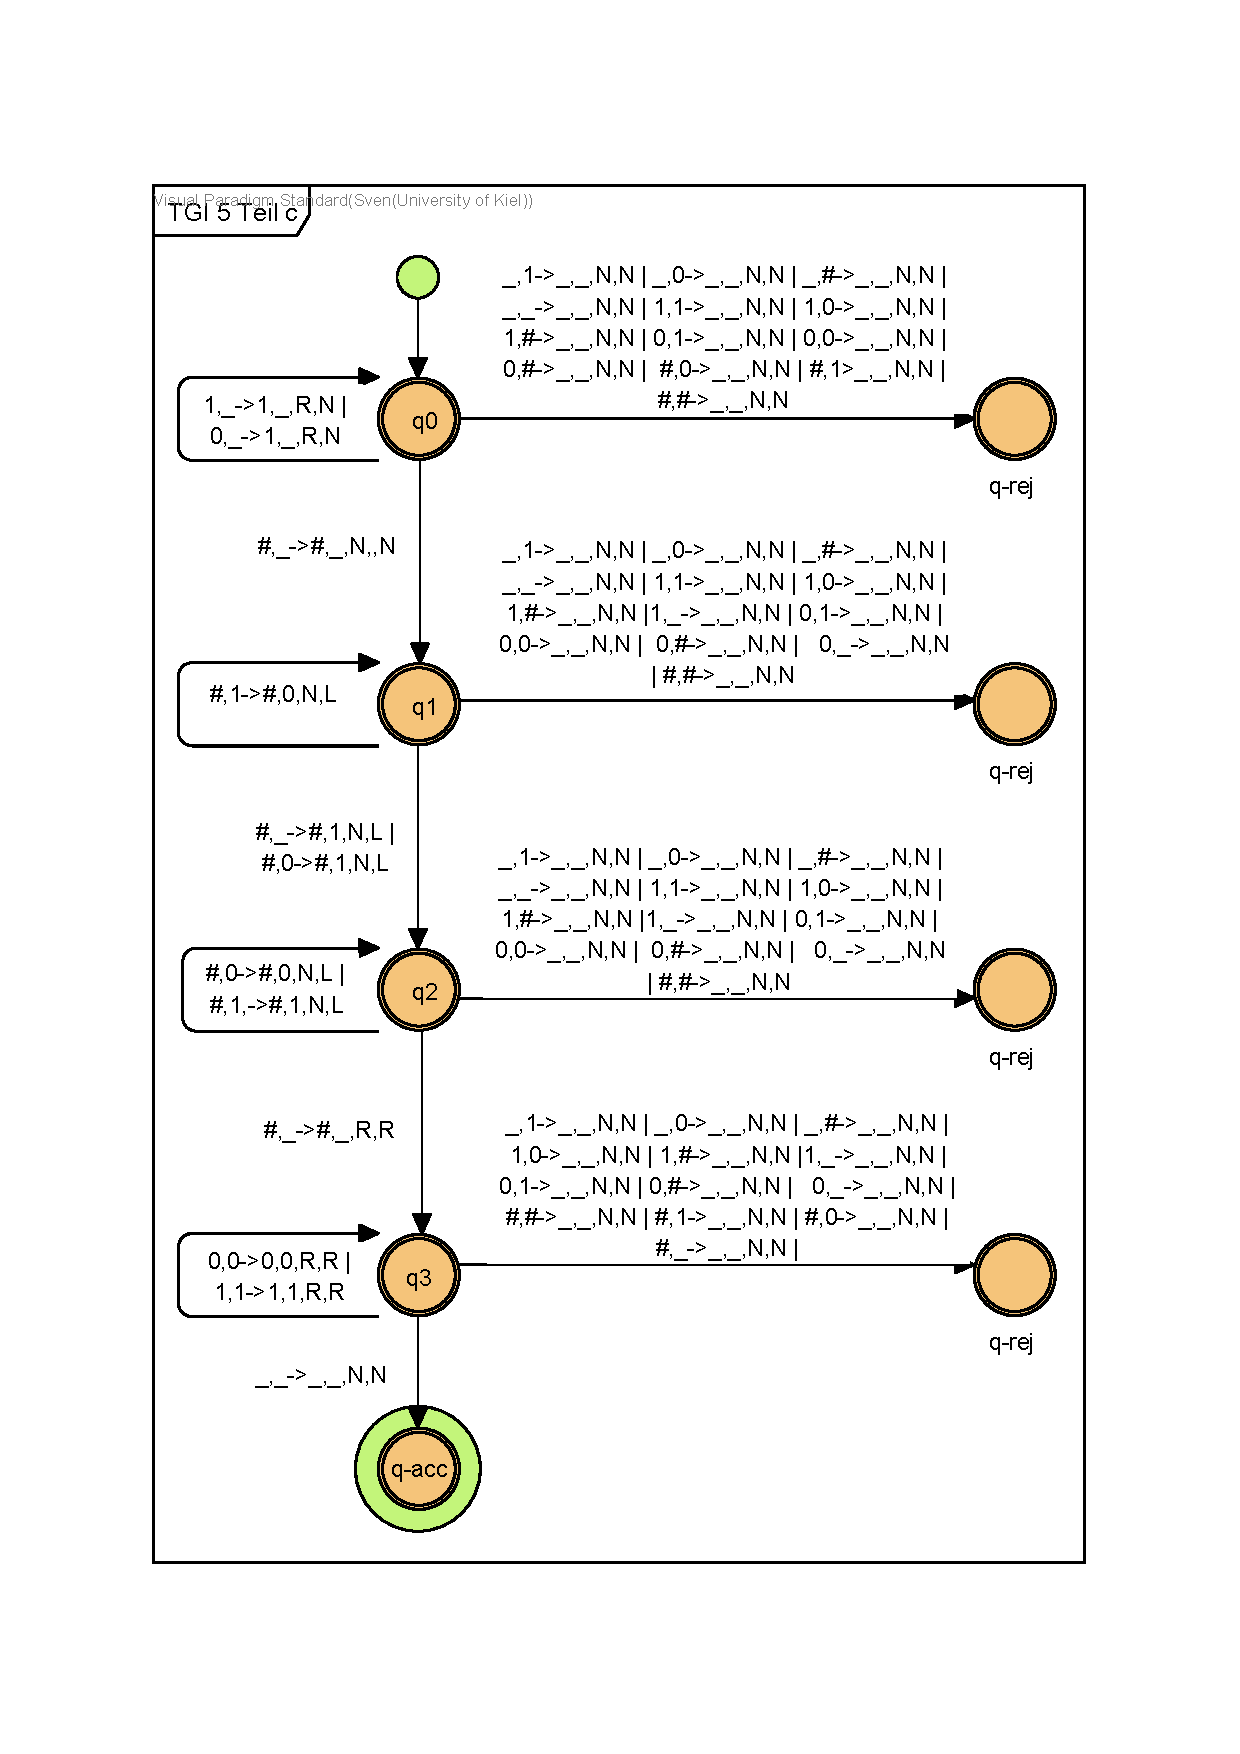
\includepdf[pages=-]{TGI_5_teil_c.pdf}

	
\end{document}